
%(BEGIN_QUESTION)
% Copyright 2006, Tony R. Kuphaldt, released under the Creative Commons Attribution License (v 1.0)
% This means you may do almost anything with this work of mine, so long as you give me proper credit

The fundamental equation for an orifice plate is based on Bernoulli's Law:

$$z_1 \rho g + {v_1^2 \rho \over 2} + P_1 = z_2 \rho g + {v_2^2 \rho \over 2} + P_2$$

$$\includegraphics[width=15.5cm]{i00731x01.eps}$$

Assuming the same height at both measuring points $z_1$ and $z_2$, Bernoulli's equation simplifies to this:

$${v_1^2 \rho \over 2} + P_1 = {v_2^2 \rho \over 2} + P_2$$

Collecting like terms to either side of the equation:

$$P_1 - P_2 = {v_2^2 \rho \over 2} - {v_1^2 \rho \over 2}$$

$$\Delta P = {\rho \over 2}({v_2^2 - v_1^2})$$

$${{2 \Delta P} \over \rho} = {v_2^2 - v_1^2}$$

If we know that the vena contracta velocity is substantially greater than the full-diameter pipe velocity, we may express the equation as an approximation:

$${{2 \Delta P} \over \rho} \approx v_2^2$$

$$v_2 \approx \sqrt{{2 \Delta P} \over \rho}$$

We know that $v_2$, in turn, directly relates to flow ($Q$), and so we may write this as an equation once more using a proportionality constant $k$ to incorporate all sizing variables and coefficients:

$$Q = k \sqrt{{\Delta P} \over \rho}$$

Based on this equation, determine what a differential pressure transmitter will do if the fluid going through an orifice plate suddenly becomes {\it denser} without changing volumetric flowrate (i.e. the velocity $v$ through the pipe remains the same while $\rho$ increases).

\underbar{file i00731}
%(END_QUESTION)





%(BEGIN_ANSWER)

If $\rho$ increases without any change in $v$, the differential pressure $\Delta$P will increase.

\vskip 10pt

If $\rho$ doubles, $\Delta$P will double as well.  However, we would actually need the $\Delta$P to increase by a factor of {\it four (4)} in order to represent a doubling of flowrate, since the $\Delta$P is customarily square-rooted to linearize the nonlinear behavior of the orifice plate.  As it is, a doubling of fluid density will only cause the indicated flow rate to increase by a factor of $\sqrt{2}$.  ``Close, but no cigar,'' as the saying goes.

%(END_ANSWER)





%(BEGIN_NOTES)


%INDEX% Measurement, flow: orifice plate

%(END_NOTES)


